\chapter{Introduction}

\section{Problem Statement}
This is usually an introduction and problem statement. It can be called something more exciting and descriptive than ``Introduction'', perhaps? 

When you quote use the correct symbols as above for quotation marks!

This is where your essay starts. Please remember that it must be 25 pages from here on. This is the first paragraph. 

The is the second paragraph. Always move to the next paragraph by leaving an open line and never using the double backslash (\verb|\\|)
command. Those are reserved for arrays, tables, and so on.

Paragraphs are separated by blank lines in the \LaTeX\ code, and we set the line spacing, paragraph indentation,
and paragraph spacing in the preamble for you, according to AIMS house style.

\section{Moving On}
Let's look at bandwidth as in Fig. \ref{bandwidth} bit. Just to demonstrate a figure!

\begin{figure}[!h]
% Use "\centering" in floats (figure, table), but if you need to center
% some text (why?) use "\begin{center}...\end{center}".
\centering 
% Figure environments same as 0.8 * \textwidth please
% That does not necessarily mean the actual picture size,
% it is a guideline for the environment which could contain
% 2 or more pictures! Be consistent and follow the guidelines
% provided in your sources.
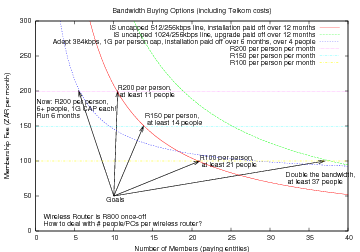
\includegraphics[width=0.8\textwidth]{images/bandwidth-colour.png}
\caption{Planning community bandwidth sharing costs. 
  Note caption capitalization.}
\label{bandwidth} 
% if you move the label it breaks the reference numbering; 
% always have it *after* the caption.
\end{figure}

\section{Bleah}
See Fig. \ref{bandwidth} to understand how figures work. It's OK to have figures on another page if you reference them correctly! if you use someone else's pictures, acknowledge them. And remember to check on the copyright. You can include tables in the same way but with the \verb|\begin{tabular}| and
 \verb|\end{tabular}| commands.

Remember how to include code with verbatim and to fix the tabs in python in a verbatim environment? It is by far best to have an include command for your code, not to re-edit it all the time!
\verbatimtabinput{code/mycode.py}

\section{Consistency}
Consistency is by far the most important thing to remember. Just after honesty and citing the work of others correctly as in \cite{AD92, Beardon}.
